\documentclass[11pt]{article}

% load some asm stuff -
\usepackage{amssymb}
\usepackage{amsmath}
\usepackage{amsthm}
%\usepackage{palatino,lettrine}
\usepackage{fancyhdr}
\usepackage{epsfig}
\usepackage[round,comma,sort]{natbib}
\usepackage{simplemargins}
\usepackage{setspace}
\usepackage{wrapfig}
\usepackage{hyperref}
%\usepackage{boiboites}
\usepackage[margin=0pt,font=small,labelfont=bf]{caption}
\newcommand{\boldindex}[1]{\textbf{\hyperpage{#1}}}
\usepackage{makeidx}\makeindex
\bibliographystyle{plos2015}


\usepackage{algpseudocode}
\usepackage{algorithm}

% Set the size
%\textwidth = 6.75 in
%\textheight = 9.75 in
%\oddsidemargin = 0.0 in
%\evensidemargin = 0.0 in
%\topmargin = 0.01 in
%\headheight = 0.0 in
%\headsep = 0.25 in
%\parskip = 0.15in
% \doublespace
\setallmargins{1in}

\newtheorem{example}{Example}[section]
\newtheorem{thm}{Theorem}[section]
\newtheorem{property}{Property}[section]

\theoremstyle{definition}
\newtheorem{defn}[thm]{Definition}

\makeatletter
% \renewcommand\subsection{\@startsection
% 	{subsection}{2}{0mm}
% 	{-0.05in}
% 	{0.1\baselineskip}
% 	{\normalfont\normalsize\bfseries}}
\renewcommand\subsubsection{\@startsection
	{subsubsection}{2}{0mm}
	{-0.05in}
	{-0.5\baselineskip}
	{\normalfont\normalsize\itshape\bfseries}}
\renewcommand\paragraph{\@startsection
	{paragraph}{2}{0mm}
	{-0.05in}
	{-0.5\baselineskip}
	{\normalfont\normalsize\itshape}}
\makeatother
\linespread{1.1}

\fancypagestyle{proposal}{\fancyhf{}%
	\fancyhead[RO,LE]{\thepage}%
	\fancyhead[LO,RE]{CHEME 131 Module 3 STRIPS}%
	\renewcommand\headrulewidth{1pt}}
\pagestyle{proposal}

\usepackage{mdframed}
\definecolor{lgray}{rgb}{0.92,0.92,0.92}
\definecolor{antiquewhite}{rgb}{0.98,0.92,0.84}
\definecolor{lightskyblue}{rgb}{0.93,0.95,0.99}

% defn environment
\mdfdefinestyle{theoremstyle}{% 
    linecolor=black,linewidth=1pt,% 
    frametitlerule=true,% 
    frametitlebackgroundcolor=lgray, 
    innertopmargin=\topskip,} 
\mdtheorem[style=theoremstyle]{definition}{Definition}

% concept environment
\mdfdefinestyle{conceptstyle}{% 
    linecolor=black,linewidth=1pt,% 
    frametitlerule=true,% 
    frametitlebackgroundcolor=lightskyblue, 
    innertopmargin=\topskip,} 
\mdtheorem[style=conceptstyle]{concept}{Concept}
\newcommand{\newterm}[1]{{\it #1}}

% Single space'd bib -
\setlength\bibsep{0pt}

\renewcommand{\rmdefault}{phv}\renewcommand{\sfdefault}{phv}
%\newboxedtheorem[boxcolor=black, background=gray!5,titlebackground=orange!20,titleboxcolor = black]{color_box_example}{Example}{test}

% Change the number format in the ref list -
\renewcommand{\bibnumfmt}[1]{#1.}

% Change Figure to Fig.
\renewcommand{\figurename}{Fig.}
\usepackage{enumitem}
\setlist{noitemsep} % or \setlist{noitemsep} to leave space around whole list

%Joycelyn Chan, Joshua Lequieu, Michael Paull, Chidanand Balaji, Ryan Tasseff
%Our derivation follows closely the earlier development of Fredrickson \citep{Fredrickson:1976fk}.

% Begin ...
\begin{document}

%\begin{titlepage}
{\par\centering\textbf{\Large CHEME 131 Module 3: Registered Interest and Principal of Securities (STRIPS) Bonds}}
\vspace{0.2in}
{\par \centering \large{Jeffrey D. Varner}}
\vspace{0.05in}
{\par \centering \large{Smith School of Chemical and Biomolecular Engineering}}
{\par \centering \large{Cornell University, Ithaca NY 14853}}
% \vspace{0.1in}
% {\par \centering \small{Copyright \copyright\ Jeffrey Varner 2018. All Rights Reserved.}}\\

%\end{titlepage}
\date{}
\thispagestyle{empty}

\setcounter{page}{1}

\section*{Introduction}
\href{https://en.wikipedia.org/wiki/United_States_Treasury_security#STRIPS}{Registered Interest and Principal of Securities (STRIPS) bonds} are a 
unique type of fixed-income investment instrument that provides investors with an alternative way to access the coupon payments of 
Treasury securities. STRIPS bonds are created by separating a Treasury securities coupon and principal components and trading them as individual 
zero-coupon securities. This process allows investors to purchase and trade the coupon or principal components separately, 
providing greater flexibility in managing their investment portfolios.

\begin{figure}[h]
    \centering
    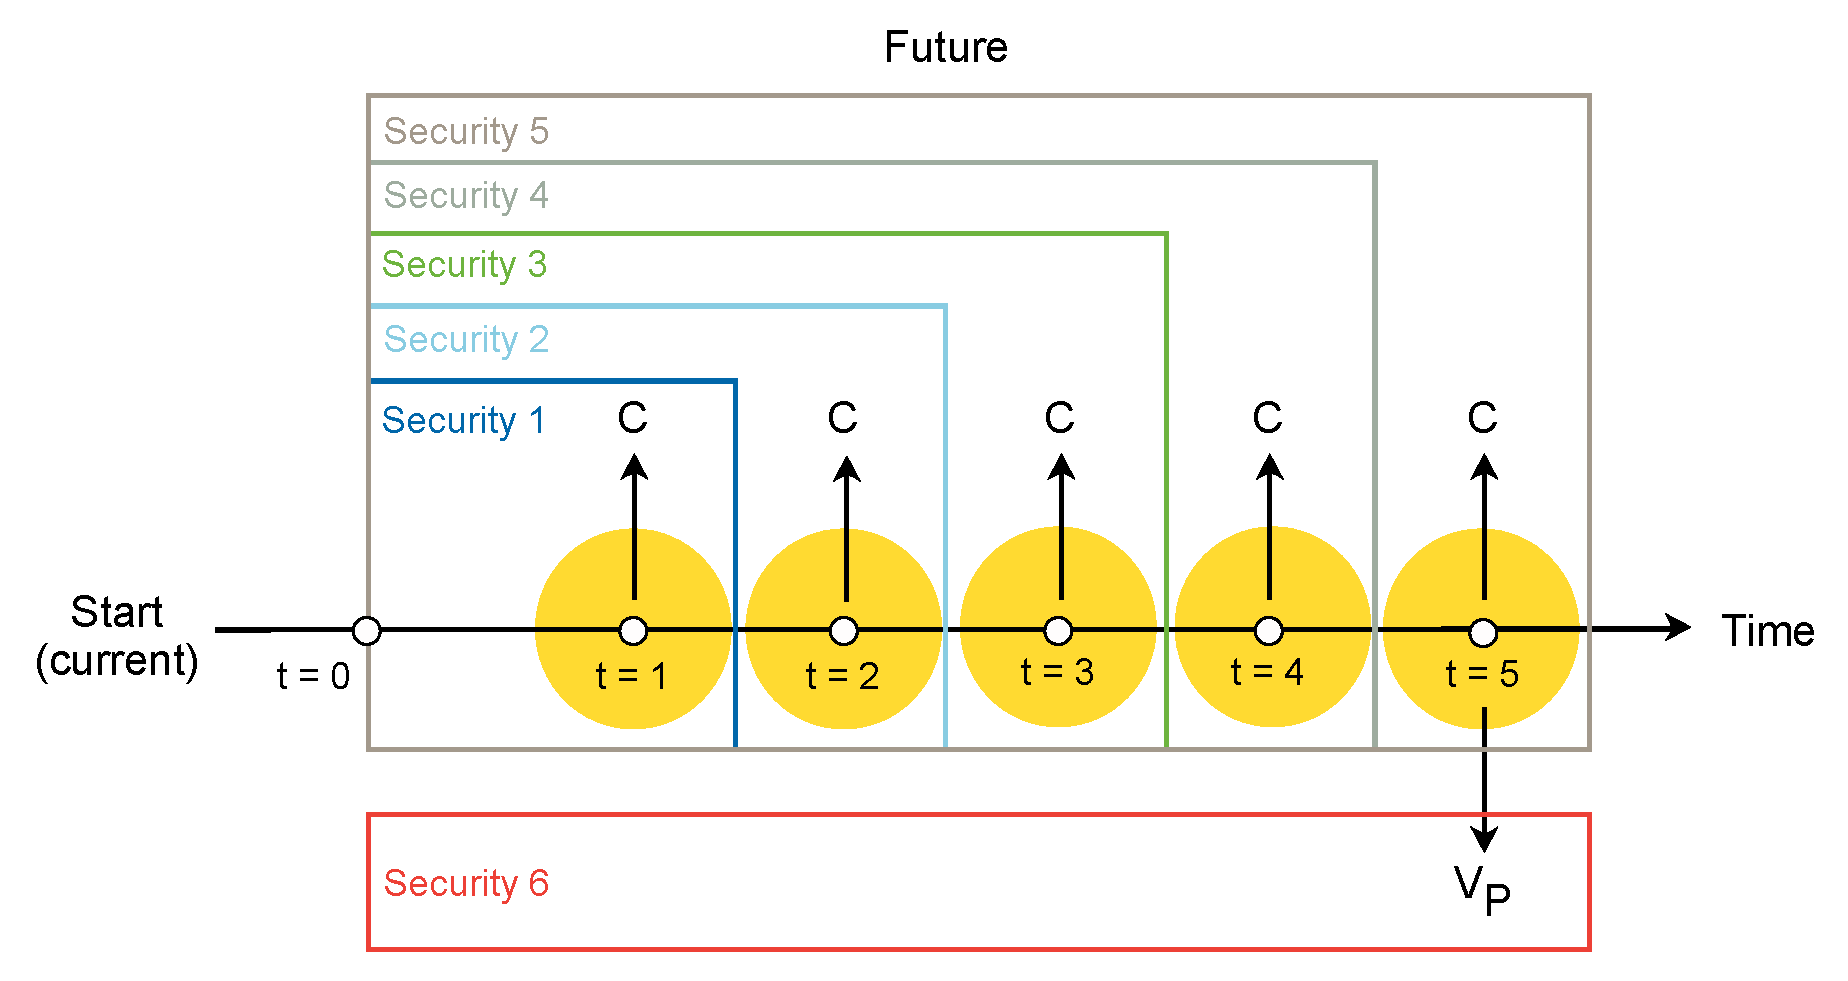
\includegraphics[width=0.85\textwidth]{./figs/Fig-STRIPS-Schematic.pdf}
    \caption{Schematic of a Registered Interest and Principal of Securities (STRIPS) bond generated from a 5-year Treasury note. The coupon and principal payments from the coupon-based 
	note are stripped from the original instrument and sold as separate marketable securities.}\label{fig:strips-bond-schematic}
\end{figure}

For example, a 5-year Treasury note with annual coupon payments of $C$ USD and a face (par) value of $V_{P}$ (USD)
can be stripped into six separate zero-coupon securities, i.e., five zero-coupon bonds, each with face values of $C$ 
and maturity of $T$= 1,2,3,4 and 5 years, and a six security with face  (par) value of $V_{P}$ USD with a duration of $T$ = 5 years (Fig. \ref{fig:strips-bond-schematic}). 
In the general case, a treasury note or bond with $N=\lambda{T}$ coupon payments, where $T$ denotes the maturity in years, and $\lambda$ represents 
the number of coupon payments per year can be stripped into $N+1$ separate zero-coupon securities.
Beyond their immediate value as investment tools, STRIPS are interesting as they provide a look at the 
\href{https://www.federalreserve.gov/data/yield-curve-models.htm}{term structure of interest rates}, i.e., the relationship between the remaining time-to-maturity of debt securities 
and the yield on those securities.

In this module, we'll explore the mathematics of STRIPS bonds and how they can be used to understand the term structure of interest rates, i.e., how we can use STRIPS to compute the short rates and the yield curve.

\section*{Spot, Short and Forward Rates}
A spot rate is the annual interest rate to be used for discounting the cash flows that occur at that date, i.e., now. Alternatively, the spot rate is the rate of return on a zero coupon bond purchased today and maturing at some future date. Suppose a bond with a face value of $V_{P}$ (future USD) and a maturity of $T$ years is purchased today for $V_{B}$ (USD). The spot rate, $\bar{r}$, is the interest rate that makes the future face value of the bond equal to the purchase price, i.e.,
\begin{equation}
V_{B}\cdot(1+\bar{r})^{T} = V_{P}
\end{equation}
where we have assumed one compounding event per year. Given the spot rate, we can compute the price of a bond with a face value of $V_{P}$ (USD) and a maturity of $T$ years, or we can compute the spot rate $\bar{r}$ from the market price of a bond $V_{B}$:
\begin{equation}
\bar{r} = \left(\frac{V_{P}}{V_{B}}\right)^{\frac{1}{T}}-1
\end{equation}
Thus, the spot rate $\bar{r}$ is constant for the entire bond life, which is a source of risk for the bondholder.
Why? Because we know that interest rates change over time. Thus, let's take a more nuanced view of the spot rate as a function of time. This context gives us the short rate.

The short rate is the interest rate between two consecutive periods, i.e., the interest rate between time $t$ and time $t+1$. We denote the short rate between period $t$ and $t+1$ as $r_{t+1,t}$. The short rate is a random variable that fluctuates in time. We've seen the short rate before in another guise, i.e., in the multiperiod discrete discount factor, $D_{t,0}$, which is the discount factor between time $t = 0$ and $t = t$ when we assume the 
interest rate, i.e., the short rate, changes in each period. Of course, the short rates are related to the spot rate, $\bar{r}$, by the following relationship:
\begin{equation}
\prod_{j=0}^{t-1}\left(1+r_{j+1,j}\right) = \left(1+\bar{r}\right)^{t}
\end{equation}
where the product on the right-hand side is the discount factor between time $t = 0$ and $t = t$.
This must be true; otherwise, we could make money by borrowing at the short rate and investing at the spot rate.

Finally, the forward rate is the expectation of the short rate between two time periods, i.e., the expected interest rate between time $t-1$ and time $t$, given the information available at time $t-1$. 
The forward rate between period $j-1\rightarrow{j}$ is denoted by $f_{t,t-1}$ and is related to the short rate by the relationship:
\begin{equation}
	f_{t,t-1} = \mathbb{E}_{t}\left[r_{t,t-1}\right]
\end{equation}

\section*{STRIPS and the Yield Curve}
The yield curve plots the yields (vertical axis) on debt securities as a function of the security's maturity (horizontal axis). 
There are three primary yield curve shapes: normal, inverted, and flat (Fig. \ref{fig:yield-curve-schematic}).
The yield curve is helpful for fixed-income investors, providing a snapshot of the market's expectations for future interest rates, and by extension inflation rates. The yield curve is also used as a benchmark for other interest rates, such as mortgage or bank lending. The yield curve is typcially constructed from observed prices and spot rates, but these quantities can be described as functions of the short rates. 

Typically, the yield on longer-term securities is higher than on shorter-term securities. This is because investors expect to be compensated for the additional risk of holding a security for longer. However, the yield curve can also be inverted, i.e., the yield on longer-term securities is lower than on shorter-term securities. This is a sign that the market expects interest rates to fall in the future. The yield curve can also be flat, i.e., the yield on longer-term securities is the same as on shorter-term securities. This indicates that the market expects interest rates to remain the same.

\begin{figure}[h]
    \centering
    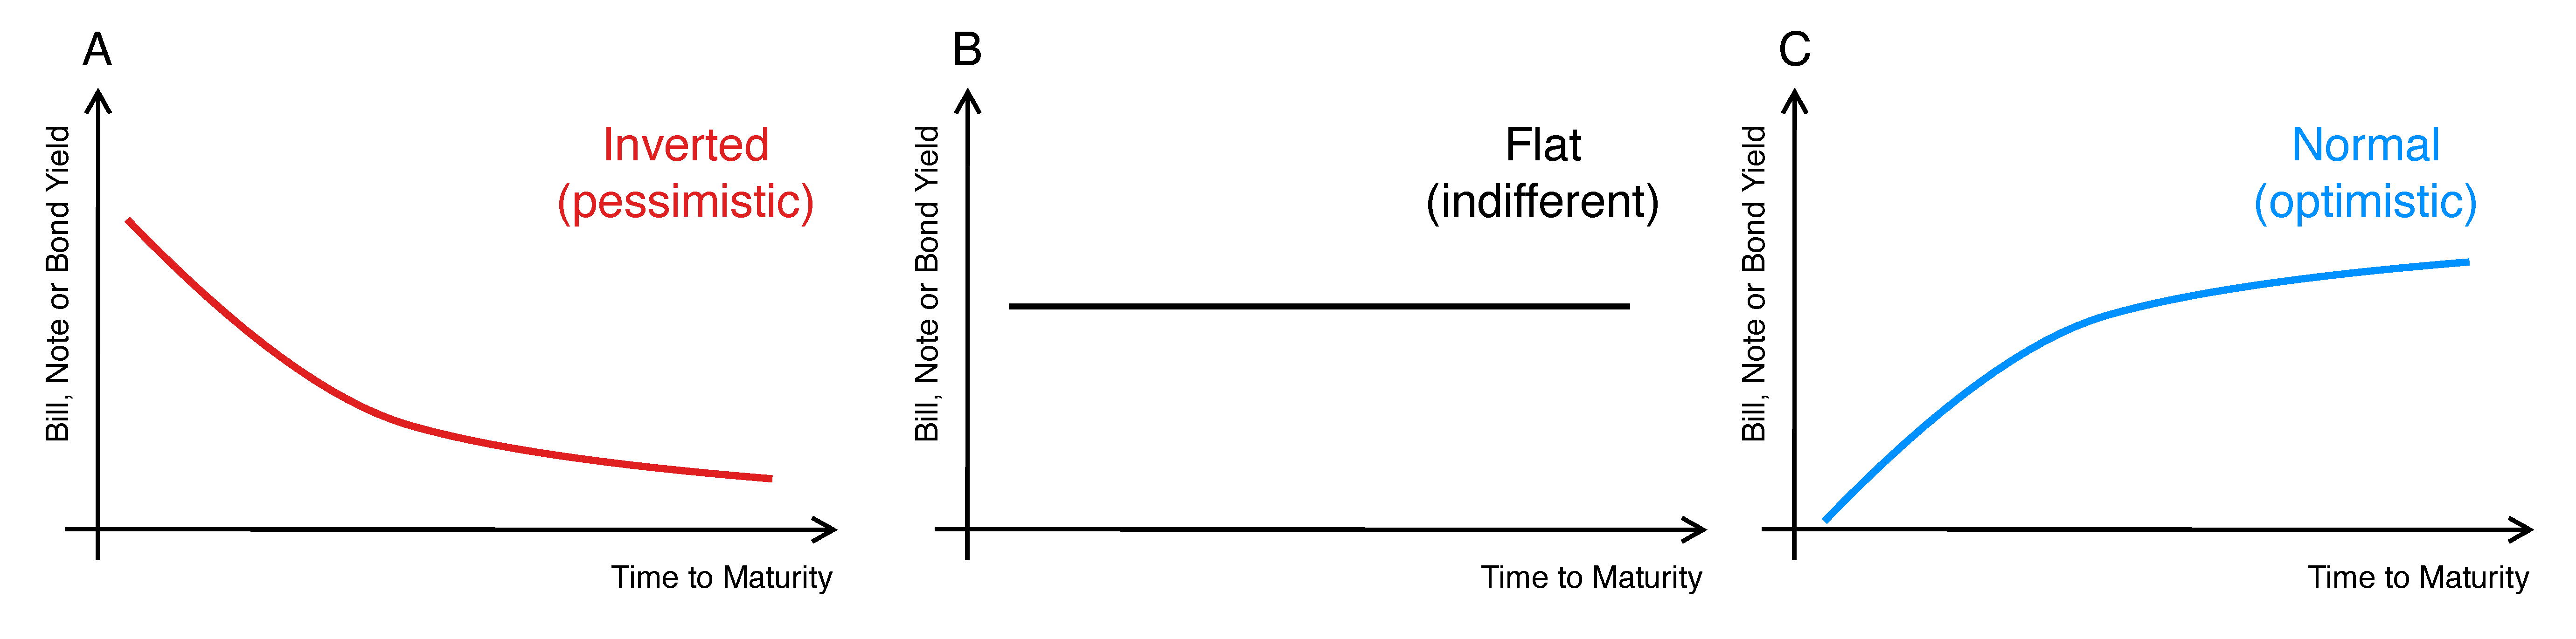
\includegraphics[width=0.95\textwidth]{./figs/Fig-YieldCurve-Schematic.pdf}
    \caption{Schematic of the regimes of the yield curve. 
	\textbf{A}: An inverted yield curve. In the inverted regime, the yield on short-term instruments is higher than long maturity; an inverted yield is indicative of a pessimistic market outlook.
	\textbf{B}: A flat yield curve. In the flat regime, the yield on short- and long-maturity bills, notes or bonds is equal; a flat regime is indicative an indifferent market outlook. 
	\textbf{C}: A normal yield curve. In the normal regime, the yield on short-term instruments is less than long maturity instruments; a normal yield is indicative of an optimistic market outlook. 
	}\label{fig:yield-curve-schematic}
\end{figure}

\section*{STRIPS pricing}
STRIPS are sold at a discount compared to their face value. However, it's essential to understand that the secondary seller, i.e., the brokerage splitting the original note or bond, determines the discount in the secondary treasury market by setting the price of the zero-coupon instrument. Let's imagine we have a set of STRIPS zero-coupon bonds with maturities $T_{1}, T_{2},\ldots, T_{N}$ years. 
We can use the prices of these STRIPS to estimate the short rates, $r_{j+1,j}$, between periods $j\rightarrow{j+1}$.
Alternatively, we can use the short rates to price the STRIPS products. 
To better understand this, let's propose three hypothetical pricing schemes that a brokerage might employ to price the zero-coupon instruments:
\begin{enumerate}
\item{\textbf{Scheme 1 constant yield}: In this approach, the brokerage prices the zero-coupon instruments to have a constant yield $\bar{r}$. This can be achieved by setting the price as an escalating fraction of the par value $V_{B} = \left(\alpha\right)^{T}\cdot{V}_{P}$, where $\alpha\leq{1}$, and $T$ represent the time to maturity of the generated zero coupon bond.}
\item{\textbf{Scheme 2 constant discount}: In this approach, the brokerage prices the zero-coupon instruments to have a constant discount, i.e., the price ratio to the face value is constant across all instruments. In this case, $V_{B} = \left(\alpha\right)\cdot{V}_{P}$ is not a function of the time to maturity of the instrument, and $\alpha\leq{1}$.}
\item{\textbf{Scheme 3 increasing yield}: In this approach, the brokerage prices the zero-coupon instruments to have an increasing yield as a function of maturity, i.e., the ratio of the price to the face value decreases with the time to maturity of the instrument.}
\end{enumerate}

\subsection*{Scheme 1: Constant Yield}
In this case, the price of the zero-coupon bond is given by $V_{B, i} = \left(\alpha\right)^{T_{i}}\cdot{V}_{P, i}$, where $\alpha\leq{1}$, and $T_{i}$ represent the time to maturity of the $ith$ generated zero coupon bond. However, this pricing expression can be rewritten as:
\begin{equation}
\left(\alpha\right)^{T_{i}} = \frac{V_{B,i}}{V_{P,i}} = \frac{1}{\left(1+\bar{r}\right)^{T_{i}}}
\end{equation}
where we can use to solve for the spot rate in terms of the escalating factor $\alpha$:
\begin{equation}
\bar{r} = \frac{1}{\alpha} - 1
\end{equation}
Thus, the spot rate is a function of the escalating factor $\alpha$, but under this pricing scheme, 
the spot rate is constant for all maturities. Thus, the yeild curve is flat for this pricing scheme.

\subsection*{Scheme 2: Constant Discount}
In this case, the ratio of the price to the face value is constant across all instruments, i.e., $V_{B, i} = \left(\alpha\right)\cdot{V}_{P, i}$, where $\alpha\leq{1}$. However, this pricing expression can be rewritten as:
\begin{equation}
\alpha = \frac{V_{B,i}}{V_{P,i}} = \frac{1}{\left(1+\bar{r}\right)^{T_{i}}}
\end{equation}
where we can use to solve for the spot rate for STRIP $i$ in terms of the escalating factor $\alpha$:
\begin{equation}
\bar{r}_{i} = \left(\frac{1}{\alpha}\right)^{1/T_{i}} - 1
\end{equation}
In this case, the spot rate $\bar{r}_{i}$ is a function of the escalating factor $\alpha$ and the maturity $T_{i}$. 
However, under this pricing scheme, the spot rate is not constant for all maturities, i.e., it decreases as the time to maturity increases. Thus, the yeild curve is downward sloping (inverted) for this pricing scheme.

\subsection*{Scheme 3: Increasing Yield}
Suppose we are the brokerage, and the yield we are willing to sell each STRIPS bond is given by:
\begin{equation}
\bar{r}_{i} = \theta_{1}+\theta_{2}\cdot\left(i-1\right)^{\beta}
\end{equation}
where $i$ denotes the STRIPS index (which is a proxy for maturity), 
$\theta_{1}>0$ denotes the interest rate for the shortest term bond in the collection, i.e., the zero-coupon bond with maturity of six months that is generate from the first coupon payment, $\theta_{2}\geq{0}$ governs how fast the rate escalates for each new STRIPS product, i.e., for each bond of longer maturity that we sell, and $\beta$ is a sensitivity parameter. Because $\theta_{1}>{0}$ and $\theta_{2}\geq{0}$, this scheme will give an expected yield curve $\bar{r}_{i}\leq\bar{r}_{i+1}$, i.e., longer maturity instruments will have a higher-yield compared to shorter-term bonds.

\subsection*{Estimating the Spot and Short Rates from STRIPS prices}
For the moment, let's assume that we have a set of STRIPS zero-coupon bonds with maturities $T_{1}, T_{2},\ldots, T_{N}$ years, 
and have the priced these STRIPS, denoted as $V_{B, i}$, using one of the three pricing schemes described above.
We can estimate the short rates, which represent the market rate of interest between periods $j-1\rightarrow{j}$, denoted as $r_{j+1,j}$, by analyzing the prices of the various STRIPS zero coupon products based on their maturity. Using a discrete discounting model, the short rates are calculated according to the following relationship:
\begin{eqnarray}
\frac{V_{P,1}}{V_{B,1}} & = & \left(1+r_{1,0}\right) \\
\frac{V_{P,2}}{V_{B,2}} & = & \left(1+r_{2,1}\right)\cdot\left(1+r_{1,0}\right) \\
\vdots & = & \vdots \\
\frac{V_{P,N}}{V_{B,N}} & = & \prod_{i=1}^{N}\left(1+r_{i,i-1}\right)
\end{eqnarray}
where $V_{P, i}$ and $V_{B, i}$ denote the face (par) value and price of the $i^{th}$ zero-coupon bond (both of which are known). Thus, we can solve for $r_{1,0}$, then insert that into the following expression to solve for $r_{2,1}$, and so on. Systematically, we can solve for the log-transformed short rates as a system of linear algebraic equations (LAEs) of the from:
\begin{equation}
\mathbf{A}\mathbf{x} = \mathbf{b}
\end{equation}
where $x_{i} = \log\left(1+r_{i,i-1}\right)$, $b_{i} = \log\left(V_{P,i}/V_{B,i}\right)$ and $\mathbf{A}$ is a lower-triangular matrix of 1's. We solve for the log-transformed short rates using back/forward substitution
and then transform these back to linear coordinates for each period: $r_{i,i-1} = 10^{x_{i}} - 1$.

\section*{Summary}
In this module, we've explored the mathematics of STRIPS bonds and how they can be used to understand the term structure of interest rates, i.e., how we can use STRIPS to compute the short rates and the yield curve. We've also explored two hypothetical pricing schemes that a brokerage might employ to price the zero-coupon instruments and how these pricing schemes affect the spot rate. 

\end{document}
